\section{Simulation d'un système de freinage sans ABS}
Durant la pratique des travaux sur VHDL-AMS il est demandé aux étudiants de réaliser et d'instancier étapes par étapes les différentes partie d'un système de freinage d'une voiture. Pour la réalisation du travail nous avons travailler avec le logiciel ModelSim et un éditeur de texte pour venir rédiger, en VHDL, les différentes instances du véhicule jusqu'à l'intégration de l'ABS.

Il est demandé d'instancier étapes par étapes différents blocs avec leurs terminaux coresspondants, comme indiqué dans le powerpoint de présentation du TP.
\begin{figure}[h]
    \centering
    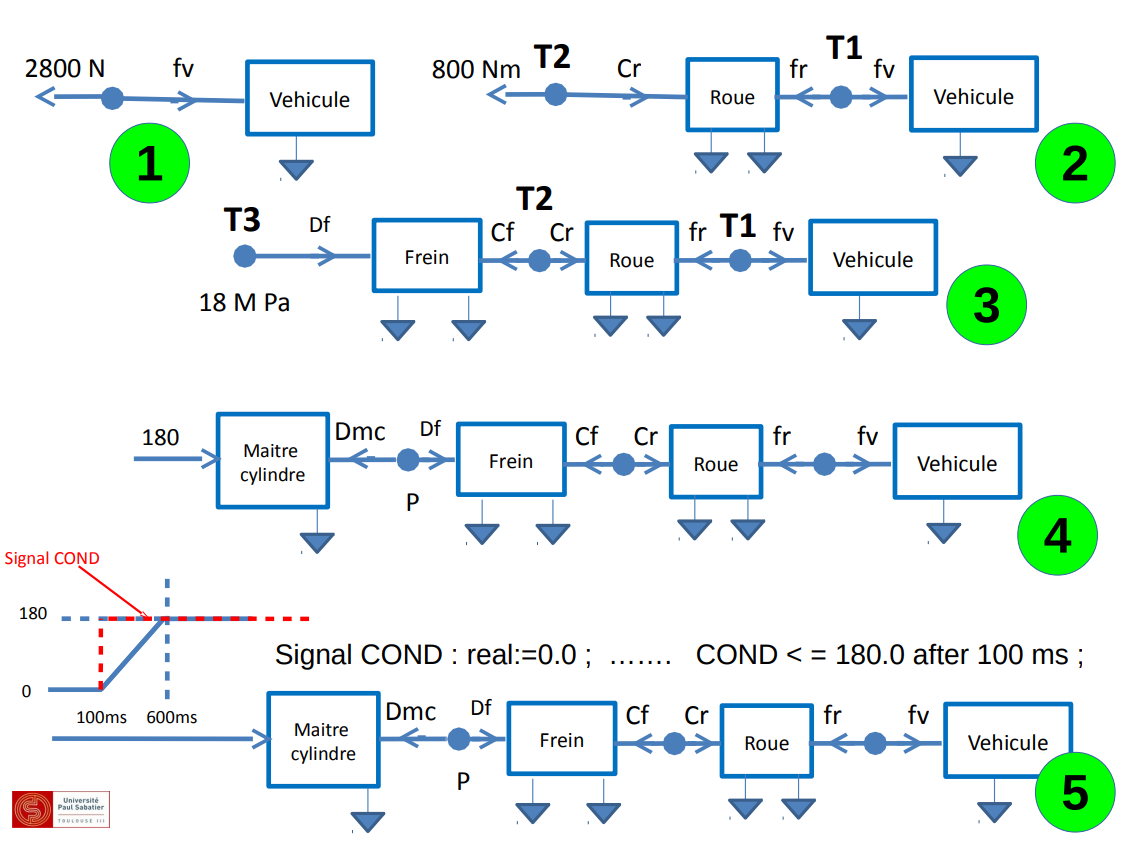
\includegraphics[width=\textwidth]{images/etapes.png}
    \caption{Implémentation des différentes parties du système de freinage d'une voiture}
\end{figure}

\subsection{Analyse instanciation véhicule }
a
\subsection{Analyse instanciation roue}
a
\subsection{Analyse instanciation frein}
a
\subsection{Analyse instanciation maître cylindre}
a
\subsection{Modélisation du régulateur de pression}
a
\newpage